
% This LaTeX was auto-generated from MATLAB code.
% To make changes, update the MATLAB code and republish this document.

\documentclass{article}
\usepackage{graphicx}
\usepackage{color}

\sloppy
\definecolor{lightgray}{gray}{0.5}
\setlength{\parindent}{0pt}

\begin{document}

    
    

\section*{24. Rational best approximation}

\begin{verbatim}
ATAPformats
\end{verbatim}
\begin{par}
Chapter 10 considered best or ``minimax'' approximation by polynomials, that is, approximation in the $\infty$-norm, where optimality is characterized by an equioscillating error curve.   This chapter presents analogous results for approximation by rational functions.  Much remains the same, but a crucial new feature is the appearance in the equioscillation condition of a number known as the \textit{defect}, which leads to the phenomenon of square blocks of degenerate entries in the ``Walsh table'' of best approximations.   This complication adds a fascinating new ingredient to the theory, but it is a complication with destructive consequences in terms of the fragility of rational approximations and the difficulty of computing them numerically.  An antidote to some such difficulties may be the use of algorithms based on linearized least-squares and the singular value decomposition, a theme we shall take up in Chapters 26 and 27.
\end{par} \vspace{1em}
\begin{par}
Another new feature in rational approximation is that we must now be careful to distinguish real and complex situations, because of a curious phenomenon: best rational approximations to real functions are in general complex.  This effect is intriguing, but it has little relevance to practical problems, so for the most part we shall restrict our attention to approximations in the space ${\cal R}_{mn}^{\hbox{\scriptsize\kern.1em real}}$ consisting of functions in ${\cal R}_{mn}$ with real coefficients.
\end{par} \vspace{1em}
\begin{par}
We will first state the main theorem, then give some examples, and then present a proof. To begin the discussion, we must define the defect. Suppose $r\in {\cal R}_{mn}$, that is, $r$ is a rational function of type $(m,n)$.  As discussed in the last chapter, this means that $r$ can be written as a fraction $p/q$ in lowest terms with $p$ and $q$ having exact degrees $\mu\le m$ and $\nu \le n$. The \textit{defect} $d$ of $r$ in ${\cal R}_{mn}$ is the number between $0$ and $n$ defined by $$ d = \min \{m-\mu, n-\nu\} \ge 0. \eqno (24.1) $$ Note that $d$ is a measure of how far \textit{both} the numerator and the denominator degrees fall short of their maximum allowed values.  Thus $(1-x^2)/(1+x^2)$, for example, has defect $0$ in ${\cal R}_{22}$ or ${\cal R}_{23}$ and defect $1$ in ${\cal R}_{33}$.
\end{par} \vspace{1em}
\begin{par}
A special case to be noted is the situation in which $r=0$, that is, $r$ is identically zero.  Recall that in this case we defined $\mu = -\infty$ and $\nu = 0$, so that $r$ is said to have exact type $(-\infty,0)$.  The definition (24.1) remains in force in this case, so if $r=0$, we say that $r$ has defect $d=n$ in ${\cal R}_{mn}$, regardless of $m$.
\end{par} \vspace{1em}
\begin{par}
The reason why defects matter has to do with the counting of zeros. Suppose $r = p/q\in {\cal R}_{mn}$ has exact type $(\kern 1pt\mu,\nu)$ and $\tilde r = \tilde p/\tilde q$ is another function in ${\cal R}_{mn}$. Then we have $$ r-\tilde r = {p\over q} - {\tilde p\over \tilde q}  = {p\tilde q - \tilde p q \over q\tilde q}, $$ a rational function of type $(\max\{\mu+n, m+\nu\},n+\nu)$.  By (24.1), this implies that $r-\tilde r$ is of type $(m+n-d,2n-d\kern .7pt )$.  Thus $r-\tilde r$ can have at most $m+n-d$ zeros, and this zero count is a key to equioscillation and uniqueness results.
\end{par} \vspace{1em}
\begin{par}

Here is our main theorem.  The study of rational best approximations goes
back to Chebyshev [1859], including the idea of equioscillation, though
without a precise statement of what form an alternant must take.
Existence was first proved by de la Vall\'ee
Poussin [1911] and Walsh [1931], and equioscillation is due
to Achieser [1930].

\end{par} \vspace{1em}
\begin{par}

{\em {\bf Theorem 24.1. Equioscillation characterization of best
approximants.} A real function $f\in C([-1,1])$ has a unique best
approximation $r^* \in {\cal R}_{mn}^{\hbox{\scriptsize\rm\kern.1em real}}$, and
a function $r \in {\cal R}_{mn}^{\hbox{\scriptsize\rm\kern.1em real}}$ is equal
to $r^*$ if and only if $f-r$ equioscillates between at least $m+n+2-d$
extreme points, where $d$ is the defect of $r$ in ${\cal R}_{mn}$.}

\end{par} \vspace{1em}
\begin{par}

``Equioscillation'' here is defined just as in Chapter 10.  For $f-r$ to
equioscillate between $k$ extreme points means that there exists a set of numbers $-1
\le x_1 < \cdots < x_k \le 1$ such that $$ f(x_j) - r(x_j) = (-1)^{j+i}
\|f-r\| , \qquad 1 \le j \le k $$ with $i = 0$ or $1$.  Here and
throughout this chapter, $\|\cdot\|$ is the supremum norm.

\end{par} \vspace{1em}
\begin{par}
We now give some examples.  To begin with, here is a function with a spike at $x=0$:
\end{par} \vspace{1em}
\begin{par}
 \vskip -2em 
\end{par} \vspace{1em}
\begin{verbatim}
x = chebfun('x'); f = exp(-100*x.^2);
\end{verbatim}
\begin{par}
Polynomial approximations of this function converge rather slowly. For example, it takes $n=20$ to achieve one digit of accuracy:
\end{par} \vspace{1em}
\begin{par}
 \vskip -2em 
\end{par} \vspace{1em}
\begin{verbatim}
[p,err] = remez(f,10);
subplot(1,2,1), hold off, plot(f-p), hold on
plot([-1 1],err*[1 1],'--k'), plot([-1 1],-err*[1 1],'--k')
FS = 'fontsize';
title('Error in type (10,0) approx',FS,9), ylim(.3*[-1 1])
[p,err] = remez(f,20);
subplot(1,2,2), hold off, plot(f-p), hold on
plot([-1 1],err*[1 1],'--k'), plot([-1 1],-err*[1 1],'--k')
title('Error in type (20,0) approx',FS,9), ylim(.3*[-1 1])
\end{verbatim}

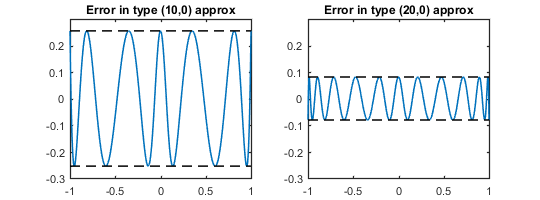
\includegraphics [width=4in]{chap24_01.png}
\begin{par}
 \vskip 1pt
\end{par} \vspace{1em}
\begin{par}
Notice that the extreme points of these error curves are distributed all across $[-1,1]$, even though the challenging part of the function would appear to be in the middle. As discussed in Chapter 16, this is typical of polynomial best approximations.
\end{par} \vspace{1em}
\begin{par}

If we switch to rational approximations, which can also be computed by
Chebfun's \verb|remez| command [Pach\'on \& Trefethen 2009, Pach\'on 2010],
the accuracy improves. Here we see error
curves for approximations of types $(2,2)$ and $(4,4)$, with much smaller
errors although the degrees are low. Note that most of the extreme points
are now localized in the middle.

\end{par} \vspace{1em}
\begin{par}
 \vskip -2em 
\end{par} \vspace{1em}
\begin{verbatim}
[p,q,rh,err] = remez(f,2,2);
subplot(1,2,1), hold off, plot(f-p./q), hold on
plot([-1 1],err*[1 1],'--k'), plot([-1 1],-err*[1 1],'--k')
title('Error in type (2,2) approx',FS,9), ylim(.1*[-1 1])
[p,q,rh,err] = remez(f,4,4);
subplot(1,2,2), hold off, plot(f-p./q), hold on
plot([-1 1],err*[1 1],'--k'), plot([-1 1],-err*[1 1],'--k')
title('Error in type (4,4) approx',FS,9), ylim(.1*[-1 1])
\end{verbatim}

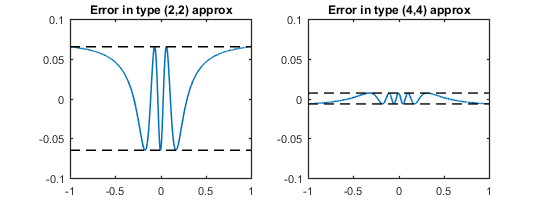
\includegraphics [width=4in]{chap24_02.png}
\begin{par}
 \vskip 1pt
\end{par} \vspace{1em}
\begin{par}
The error curves just plotted provide good examples of the role of the defect in the characterization of best approximants.  The function $f$ is even, and so are its best approximations (Exercise 24.1).  Thus we expect that the type $(2,2)$, $(3,2)$, $(2,3)$ and $(3,3)$ best approximations will all be the same function, a rational function of exact type $(2,2)$ whose error curve has 7 points of equioscillation.  For $(m,n) = (2,2)$, the defect is $0$ and there is one more equioscillation point than the minimum $m+n+2-d=6$.  For $(m,n) = (3,2)$ or $(2,3)$, the defect is $0$ and the number of equiscillation points is exactly the minimum $m+n+2-d$. For $(m,n) = (3,3)$, the defect is $1$ and the number of equiscillation points is again exactly the minimum $m+n+2-d$.
\end{par} \vspace{1em}
\begin{par}
Similarly, the error curve in the plot on the right, with 11 extrema, indicates that this rational function is a best approximation not only of type $(4,4)$ but also of types $(5,4)$, $(4,5)$, and $(5,5)$.
\end{par} \vspace{1em}
\begin{par}
Here is another example, an odd function:
\end{par} \vspace{1em}
\begin{par}
 \vskip -2em 
\end{par} \vspace{1em}
\begin{verbatim}
f = x.*exp(-5*abs(abs(x)-.3));
clf, plot(f), grid on, ylim(.4*[-1 1])
title('An odd function','fontsize',9)
\end{verbatim}

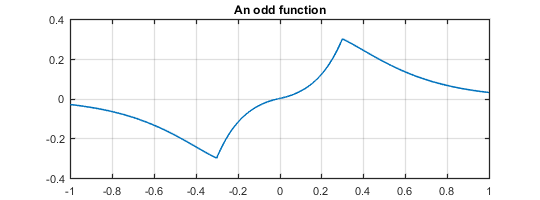
\includegraphics [width=4in]{chap24_03.png}
\begin{par}
 \vskip 1pt 
\end{par} \vspace{1em}
\begin{par}
If we look for a best approximation of type $(4,5)$, we find that the numerator has exact degree $3$:
\end{par} \vspace{1em}
\begin{par}
 \vskip -2em 
\end{par} \vspace{1em}
\begin{verbatim}
[p,q,rh,err] = remez(f,4,4); format short, chebpoly(p)
\end{verbatim}

        \color{lightgray} \begin{verbatim}ans =
    0.0000    0.0093   -0.0000    0.0314   -0.0000
\end{verbatim} \color{black}
    \begin{par}
and the denominator has exact degree $4$:
\end{par} \vspace{1em}
\begin{par}
 \vskip -2em 
\end{par} \vspace{1em}
\begin{verbatim}
chebpoly(q)
\end{verbatim}

        \color{lightgray} \begin{verbatim}ans =
    0.1174    0.0000    0.4065   -0.0000    0.3003
\end{verbatim} \color{black}
    \begin{par}
The defect is 1, so there must be at least $4+5+2-1= 10$ extreme points in the error curve.  In fact, there are exactly 10:
\end{par} \vspace{1em}
\begin{par}
 \vskip -2em 
\end{par} \vspace{1em}
\begin{verbatim}
plot(f-p./q), hold on, ylim(.04*[-1 1])
plot([-1 1],err*[1 1],'--k'), plot([-1 1],-err*[1 1],'--k')
title('Error curve of type (4,5) approximation','fontsize',9)
\end{verbatim}

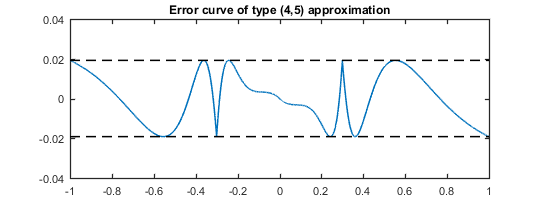
\includegraphics [width=4in]{chap24_04.png}
\begin{par}
 \vskip 1pt 
\end{par} \vspace{1em}
\begin{par}
We conclude that $r$ is the best approximation of types $(4,4), (4,5), (3,4)$ and $(3,5)$.
\end{par} \vspace{1em}
\begin{par}

Let us now turn to the proof of Theorem 24.1. For polynomial
approximations, our analogous theorem was Theorem 10.1, whose proof
proceeded in four steps:

\end{par} \vspace{1em}
\begin{par}

{\em 1. Existence proof via compactness,}
\vskip -6pt 
\end{par} \vspace{1em}
\begin{par}

{\em 2. Equioscillation $\Rightarrow$ optimality,}
\vskip -6pt 
\end{par} \vspace{1em}
\begin{par}

{\em 3. Optimality $\Rightarrow$ equisoscillation,}
\vskip -6pt 
\end{par} \vspace{1em}
\begin{par}

{\em 4. Uniqueness proof via equioscillation.}

\end{par} \vspace{1em}
\begin{par}

For rational functions, we shall follow the same sequence. The main
novelty is in step 1, where compactness must be applied in a subtler way.
We shall see an echo of this argument one more time in Chapter 27, in the proof
of Theorem 27.1 for Pad\'e approximants.

\end{par} \vspace{1em}
\begin{par}
\textit{Part 1 of proof: Existence via compactness.} For polynomial approximation, in Chapter 10, we noted that $\|f-p\|$ is a continuous function on ${\cal P}_n$, and since one candidate approximation was the zero polynomial, it was enough to look in the bounded subset $\{p\in {\cal P}_n: \|f-p\|\le \|f\|\}$. Since this set was compact, the minimum was attained.
\end{par} \vspace{1em}
\begin{par}

For rational functions, $\|f-r\|$ is again a continuous function on
${\cal R}_{mn}^{\hbox{\scriptsize\kern.1em real}}$, and again it is enough to look in the bounded subset $\{r\in
{\cal R}_{mn}^{\hbox{\scriptsize\kern.1em real}}: \|f-r\|\le \|f\|\}$, or more simply, the larger bounded set
$\{r\in {\cal R}_{mn}^{\hbox{\scriptsize\kern.1em real}}: \|r\|\le 2\|f\|\}$. The difficulty is that bounded sets
of rational functions are not in general compact.  To illustrate this
fact, consider the family of functions
$$ r_\varepsilon(x) = {x^3 + \varepsilon \over x^2+\varepsilon}, \eqno (24.2) $$
where $\varepsilon>0$ is a parameter.   For each $\varepsilon$,
$r_\varepsilon(x)$ is a continuous function on $[-1,1]$ with
$\|r_\varepsilon\|=1$.  As
$\varepsilon\to 0$, however, $r_\varepsilon$ behaves discontinuously:
$$ \lim_{\varepsilon\to 0} r_\varepsilon(x) = \cases{1 & $x=0,$\cr x & $ x\ne 0.$} $$
So we cannot find a limit function $r_0$ by taking a limit as
$\varepsilon\to 0$. What saves us, however, is that the spaces of
numerators and denominators are both compact, so we can argue that the
numerators and denominators
separately approach limits $p_0$ and $q_0$, which in this example would
be $x^3$ and $x^2$.  We then define a limiting rational function by $r_0
= p_0/q_0$ and argue by continuity that it has the necessary
properties. This
kind of reasoning is spelled out in greater generality in [Walsh 1931].

\end{par} \vspace{1em}
\begin{par}

Suppose then that $\{r_k\}$ is a sequence of functions in
$ {\cal R}_{mn}^{\hbox{\scriptsize\kern.1em real}}$ with $\|r_k\|\le 2\|f\|$ and
$$\lim_{k\to\infty} \|f-r_k\| = E =
\inf_{r\in {\cal R}_{mn}^{\hbox{\scriptsize\kern.1em real}}} \|f-r\|.$$ Write each
$r_k$ in the form $p_k/q_k$ with $p_k\in {\cal P}_m$, $q_k\in {\cal
P}_n$, $q_k(x)\ne 0$ for all $x\in [-1,1]$, and $\|q_k\| = 1$, hence
$\|p_k\|\le \|q_k\|\|r_k\| \le 2\|f\|$. Since $\{p_k\}$ and $\{q_k\}$ lie
in compact sets, we may assume by passing to a subsequence if necessary
that $p_k\to p^*$ and $q_k\to q^*$ for some $p^*\in {\cal P}_m$ and
$q^*\in {\cal P}_n$.  Since $\|q_k\|=1$ for each $k$, $\|q^*\| = 1$ too,
and thus $q^*$ is not identically zero but has at most a finite set of
zeros on $[-1,1]$. Now define $r^* = p^*/q^* \in
{\cal R}_{mn}^{\hbox{\scriptsize\kern.1em real}}$. For all $x\in[-1,1]$ except
perhaps the zeros of $q^*$, $|f(x)-r^*(x)| = \lim_{k\to\infty} |f(x) -
r_k(x)|\le E$.  By continuity, the same must hold for all $x\in [-1,1],$
with $p^*$ having zeros in $[-1,1]$ wherever $q^*$ does. Thus $r^*$ is a
best approximation to $f$. $~\hbox{\vrule width 2.5pt depth 2.5 pt height
3.5 pt}$

\end{par} \vspace{1em}
\begin{par}
\textit{Part 2 of proof: Equioscillation $\Rightarrow$ optimality.} Suppose $f-r$ takes equal extreme values with alternating signs at $m+n+2-d$ points $x_0<x_1< \cdots < x_{m+n+1-d}$, and suppose $\| f-\tilde r\| < \| f-r\|$ for some $\tilde r\in {\cal R}_{mn}^{\hbox{\scriptsize\kern.1em real}}$. Then $r-\tilde r$ must take nonzero values with alternating signs at the equioscillation points, implying that it must take the value zero in at least $m+n+1-d$ points in-between. However, as observed above, $r-\tilde r$ is of type $(m+n-d, 2n-d\kern .7pt )$.  Thus it cannot have $m+n+1-d$ zeros unless it is identically zero, a contradiction. $~\hbox{\vrule width 2.5pt depth 2.5 pt height 3.5 pt}$
\end{par} \vspace{1em}
\begin{par}

{\em Part 3 of proof: Optimality $\Rightarrow$ equisoscillation.}
Suppose $f-r$ equioscillates at fewer than $m+n+2-d$ points, and set
$E=\|f-r\|$. Without loss of generality suppose the leftmost extremum is
one where $f-r$ takes the value $-E$.  Then by a compactness
argument, for all sufficiently small $\varepsilon>0$, there are numbers $-1< x_1<
\cdots  < x_k< 1$ with $k\le m+n-d$ such that
$(f-r)(x) <E - \varepsilon$ for $x\in [-1,x_1+\varepsilon] \cup [x_2-\varepsilon,x_3+\varepsilon] \cup
[x_4-\varepsilon,x_5+\varepsilon] \cup \cdots$
and $(f-r)(x)>-E+\varepsilon$ for $x\in [x_1-\varepsilon,x_2+\varepsilon]
\cup [x_3-\varepsilon,x_4+\varepsilon] \cup \cdots.$\ \ Let
$r$ be written in the form $p/q$, where
$p$ has degree $\mu \le m-d$ and $q$ has degree $\nu \le n - d$, with $p$
and $q$ having no roots in common. The proof now consists of showing that
$r$ can be perturbed to a function $\tilde r = (\kern .7pt p+\delta p)/(q+\delta q)
\in {\cal R}_{mn}$ with the properties that $\|\tilde r - r\|<\varepsilon$ and
$\tilde r - r$ is strictly negative for $x\in [-1,x_1-\varepsilon] \cup [x_2+\varepsilon,x_3-\varepsilon]
\cup [x_4+\varepsilon,x_5-\varepsilon] \cup \cdots$
and strictly positive for $x\in [x_1+\varepsilon,x_2-\varepsilon]
\cup [x_3+\varepsilon,x_4-\varepsilon] \cup \cdots.$
Such a function $\tilde r$ will have error
less than $E$ throughout the whole interval $[-1,1]$. We calculate
$$ \tilde r = {p+\delta p\over q + \delta q} =
{(\kern .7pt p+\delta p)(q-\delta q)\over q^2 } + O(\|\delta q\|^2) $$
and therefore $$ \tilde r - r =
{q\delta p - p\delta q\over q^2 } + O(\|\delta p\|\|\delta q\| +\|\delta q\|^2). $$
We are done if we can show that $\delta p$ and $\delta q$ can be chosen
so that $q\delta p - p\delta q$ is a nonzero polynomial of degree exactly
$k$ with roots $x_1, \dots , x_k$; by scaling this $\delta p$ and $\delta q$ sufficiently
small, the quadratic terms above can be made arbitrarily small relative to the
others, so that the required $\varepsilon$ conditions are satisfied.
This can be shown by the Fredholm
alternative of linear algebra.  The map from the $(m+n+2)$-dimensional
set of choices of $\delta p$ and $\delta q$ to the
$(m+n+1-d\kern .7pt )$-dimensional space of polynomials $q\delta p - p\delta q$ is
linear. To show the map is surjective, it is enough to show that its
kernel has dimension $d+1$ but no more.  Suppose then that $q\delta p -
p\delta q$ is zero, that is, $q\delta p = p\delta q$. Then since $p$ and
$q$ have no roots in common, all the roots of $p$ must be roots of
$\delta p$ and all the roots of $q$ must be roots of $\delta q$.  In
other words we must have $\delta p = g p$ and $\delta q = g q$ for some
polynomial $g$.  Since $\delta p$ has degree no greater than $m$ and
$\delta q$ has degree no greater than $n$, $g$ can have degree no greater
than $d$. The set of polynomials of degree $d$ has dimension $d+1$, so we
are done.
$~\hbox{\vrule width 2.5pt depth 2.5 pt height 3.5 pt}$

\end{par} \vspace{1em}
\begin{par}
\textit{Part 4 of proof: Uniqueness via equioscillation.} Finally, to prove uniqueness, suppose $r$ is a best approximation whose error curve equioscillates between extreme points at $x_0 < x_1 < \cdots < x_{m+n+1-d}$, and suppose $\|f-\tilde r\| \le \|f-r\|$ for some $\tilde r\in {\cal R}_{mn}^{\hbox{\scriptsize\kern.1em real}}$. Then (without loss of generality) $(r-\tilde r)(x)$ must be $\le 0$ at $x_0, x_2, x_4,\dots$ and $\ge 0$ at $x_1, x_3, x_5,\dots .$  This implies that $r-\tilde r$ has roots in each of the $m+n+1-d$ closed intervals $[x_0,x_1], \dots, [x_{m+n-d},x_{m+n+1-d}]$, and since $r-\tilde r$ is a rational function of type $(m+n-d,2n-d\kern .7pt )$, the same must hold for its numerator polynomial. We wish to conclude that its numerator polynomial has at least $m+n+1-d$ roots in total, counted with multiplicity, implying that $r=\tilde r$. The argument for this is the same as given in the proof of Theorem 10.1. $~\hbox{\vrule width 2.5pt depth 2.5 pt height 3.5 pt}$
\end{par} \vspace{1em}
\begin{par}
We have now finished the substantial mathematics. It is time to look at some of the consequences.
\end{par} \vspace{1em}
\begin{par}
One of the recurring themes in the subject of rational approximation is the phenomenon of \textit{square blocks in the Walsh table.}  Suppose that a real function $f\in C([-1,1])$ is given, and consider the set of all of its real rational best approximations of type $(m,n)$ for various $m,n\ge 0$.  We can imagine these laid out in an array, with $m$ along the horizontal and $n$ along the vertical.  This array is called the \textit{Walsh table} for $f$ [Walsh 1934].
\end{par} \vspace{1em}
\begin{par}

Generically, all the entries in the Walsh table for a given $f$ will be
distinct, and in this case we say that $f$ is {\em normal}. Sometimes,
however, certain entries in the table may be repeated, and in fact this
is a frequent occurrence because it happens whenever $f$ is even or odd.
If $f$ is even, then for any nonegative integers $j$ and $k$, all of its
rational approximations of types $(2j,2k)$, $(2j+1,2k)$, $(2j,2k+1)$ and
$(2j+1,2k+1)$ must be the same. Similarly, if $f$ is odd, then all of its
approximations of types $(2j+1,2k)$, $(2j+2,2k)$, $(2j+1,2k+1)$ and
$(2j+2,2k+1)$ must be the same. We have already seen a number of
examples.

\end{par} \vspace{1em}
\begin{par}

More generally, repeated entries or ``degeneracies'' in the Walsh table
may take complicated forms.  Nevertheless the equioscillation condition
imposes quite a bit of structure on the chaos.  Degeneracies always
appear precisely in a pattern of square blocks. The following statement
of this result is taken from [Trefethen 1984], where a discussion of
various aspects of this and related problems can be found. We shall
return to the subject of square blocks in Chapter 27, on Pad\'e
approximation.

\end{par} \vspace{1em}
\begin{par}

{\em {\bf Theorem 24.2. Square blocks in the Walsh table.} The Walsh
table of best real rational approximants to a real rational function
$f\in C([-1,1])$ breaks into precisely square blocks containing identical
entries.  (If $f$ is rational, one of these will be infinite in extent.)
The only exception is that if an entry $r=0$ appears in the table, then
it fills all of the columns to the left of some fixed index $m = m_0$.}

\end{par} \vspace{1em}
\begin{par}
\textit{Proof.} Given a nonrational function $f$, let $r\ne 0$ be a best approximation in ${\cal R}_{\mu\nu}^{\hbox{\scriptsize\kern.1em real}}$ of exact type $(\kern 1pt\mu,\nu)$.  (The cases of rational $f$ or $r=0$ can be handled separately.)  By Theorem 24.1, the number of equioscillation points of $f-r$ is $\mu+\nu+2+k$ for some integer $k\ge 0$.  We note that $r$ is an approximation to $f$ in ${\cal R}_{mn}^{\hbox{\scriptsize\kern.1em real}}$ for any $m\ge \mu$ and $n\ge \nu$, and the defect is $\min\{m-\mu,n-\nu\}$. Thus by Theorem 24.1, $r$ is the best approximation to $f$ precisely for those values of $(m,n)$ satisfying $m\ge \mu$, $n\ge \nu$, and $\mu+\nu+2+k \ge m + n + 2 - \min\{m-\mu,n-\nu\}$. The latter condition simplifies to $n\le \nu+k$ and $m\le \mu+k$, showing that $r$ is the best approximation to $f$ precisely in the square block $\mu \le m \le \mu +k$, $\nu \le n \le \nu + k$. $~\hbox{\vrule width 2.5pt depth 2.5 pt height 3.5 pt}$
\end{par} \vspace{1em}
\begin{par}
Within a square block in the Walsh table, the defect $d$ is equal to zero precisely in the first column and the first row.  An approximation with $d=0$ is sometimes said to be \textit{nondegenerate}. It can have more points of equioscillation than the generic number $m+n+2$, but never fewer.
\end{par} \vspace{1em}
\begin{par}
As mentioned above, the theory of equioscillation and degeneracies is very appealing mathematically.  As an example we note a result due to Werner [1964], in completion of earlier work of Maehly and Witzgall [1960]: the type $(m,n)$ \textit{best approximation operator}, which maps functions $f$ to their best approximations $r_{mn}^*$, is continuous at $f$ with respect to the supremum norm if and only if $f\in {\cal R}_{mn}$ or the corresponding function $r_{mn}^*$ is nondegenerate. The essential reason for this effect is that if a function $r^*$ is the best approximation to $f$ in a nontrivial square block, then a small perturbation $f \to \tilde f$ might fracture that block into pieces of size $1\times 1$ [Trefethen 1984].  If $(m,n)$ corresponds to a degenerate position in the block, with $d>0$, then the best approximation $\tilde r^*$ for such an $\tilde f$ would need to have a higher equioscillation number than that of $r^*$ for $f$, requiring $\tilde r^*$ to be far from $r^*$ if $\|f-r^*\|$ is positive.
\end{par} \vspace{1em}
\begin{par}

These complications hint at some of the practical difficulties of
rational approximation.  For example, the Remez algorithm is based on
explicit manipulation of alternant sets.  If
the number of extremal points is not known a priori, it is plausible that
one may expect numerical difficulties in certain circumstances.  Indeed,
this is the case, and so far as I am aware, no implementation of the
Remez algorithm for rational approximation, including Chebfun's, can be
called fully robust.  Other kinds of algorithms may have better prospects.

\end{par} \vspace{1em}
\begin{par}

We finish by returning to the matter of best {\em complex\/} approximations
to real functions.   Nonuniqueness of certain complex rational
approximations was pointed out by Walsh in the 1930s.  Later Lungu [1971]
noticed, following a suggestion of Gonchar, that the nonuniqueness arises
even for approximation of a real function $f$ on $[-1,1]$, with
examples as simple as type $(1,1)$ approximation of $|x|$. (Exercise 24.3
gives another proof that there must exist such examples.)  These
observations were rediscovered independently by Saff and Varga [1978a].
Ruttan [1981] showed that complex best approximations are always better
than real ones in the strict lower-right triangle of a square block, that
is, when a type $(m,n)$ best approximation equioscillates in no more than
$m+n+1$ points. Trefethen and Gutknecht [1983a] showed that for every
$(m,n)$ with $n\ge m+3$, examples exist where the ratio of the optimal
complex and real errors is arbitrarily small. Levin, Ruttan and Varga
showed that the minimal ratio is exactly $1/3$ for $n=m+2$ and exactly
$1/2$ for $1\le n\le m+1$ [Ruttan \& Varga 1989]. None of this has much
to do with practical approximation, but it is fascinating.

\end{par} \vspace{1em}
\begin{par}

\begin{displaymath}
\framebox[4.7in][c]{\parbox{4.5in}{\vspace{2pt}\sl
{\sc Summary of Chapter 24.}
Any real function $f\in C([-1,1])$ has a unique best approximation $r^*
\in {\cal R}_{mn}^{\hbox{\scriptsize\rm\kern.1em real}}$ with respect to the
$\infty$-norm, and $r^*$ is characterized by having an error curve that
equioscillates between at least $m+n+2-d$ extreme points, where $d$ is the
defect of $r$ in ${\cal R}_{mn}$.  In the Walsh table of all best approximations
to $f$ indexed by $m$ and $n$, repeated entries, if any, lie in exactly
square blocks.\vspace{2pt}}}
\end{displaymath}

\end{par} \vspace{1em}
\begin{par}
 \small\smallskip\parskip=2pt
{\bf Exercise 24.1.  Approximating even functions.}  Prove that if a real
function $f\in C([-1,1])$ is even, then its real best approximations of all
types $(m,n)$ are even.
\par
{\bf Exercise 24.2.  Approximating the Gaussian.}  The first figures of
this chapter considered lower degree polynomial and rational
approximations of $\exp(-100 x^2)$ on $[-1,1]$.  Make a plot of the
errors in approximations of types $(n,0)$ and $(n,n)$, now taking $n$ as
high as you can.  (You may find that the {\tt cf} command takes you farther
than {\tt remez}.)   How do the polynomial and rational approximations compare?
\par
{\bf Exercise 24.3.  Complex approximations and nonuniqueness.}
(a) Suppose a real function $f\in C([-1,1])$ takes both the values $1$
and $-1$. Prove that no real rational function $r \in
{\cal R}_{0n}^{\hbox{\scriptsize\kern.1em real}}$, for any $n$, can have
$\|f-r\|<1$.
(b) On the other hand, show that for any $\varepsilon>0$, there is a
complex rational function $r \in {\cal R}_{0n}$ for some $n$ with
$\|f-r\|<\varepsilon$. (Hint: perturb $f$ by an imaginary constant and
consider its reciprocal.)
(c) Conclude that type $(0,n)$ complex rational best approximations in
$C([-1,1])$ are nonunique in general for large enough $n$.
\par
{\bf Exercise 24.4.  A function with a spike.} Plot chebfuns of the
function (24.2) for $\varepsilon = 1, 0.1, \dots, 10^{-6}$ and determine
the polynomial degree $n(\varepsilon)$ of the chebfun in each case. What
is the observed asymptotic behavior of $n(\varepsilon)$ as
$\varepsilon\to 0\kern .7pt $? How accurately can you explain this observation based
on the theory of Chapter 8?
\par
{\bf Exercise 24.5.}  $\hbox{\bf de la Vall\'ee Poussin lower bound.}$
Suppose an approximation
$r \in {\cal R}_{mn}^{\hbox{\scriptsize\kern.1em real}}$
to $f\in C([-1,1])$ approximately
equioscillates in the sense that there are points
$-1\le s_0< s_1 < \cdots < s_{m+n+1-d}\le 1$ at which $f-r$
alternates in sign with $|f(s_j)-r(s_j)| \ge \varepsilon$
for some $\varepsilon > 0$, where $d$ is the defect of $r$ in
${\cal R}_{mn}$.  Show that the best approximation
$r^* \in {\cal R}_{mn}^{\hbox{\scriptsize\kern.1em real}}$
satisfies $\|f-r^*\|\ge \varepsilon$.  (Compare Exercise 10.3.)
\par
{\bf Exercise 24.6.  A rational lethargy theorem.}
Let $\{\varepsilon_n\}$
be a sequence decreasing monotonically to $0$.
Adapt the proof of Exercise 10.7 to show that that there is a function
$f\in C([-1,1])$ such that $\|f-r_{nn}^*\|\ge \varepsilon_n$ for all $n$.
\par 
\end{par} \vspace{1em}



\end{document}
    
